%!TEX root = proj_report_outline.tex
\chapter{Requirements}\label{C:requirements}

\section{Previous Work}

To contextualise the requirements identified this section first introduces Callaghan Innovation's previous work on PitchHub. Callaghan Innovation began work on the idea of PitchHub in 2013. Since this time Callaghan Innovation has discerned what functionality a collaborative innovation platform like PitchHub needs to fulfill it's aim of driving innovation by connecting the roles identified in Section \ref{commonRolesInInnovation}.

\subsection{Pitch Cards Conceptualisation}
As discussed in Chapter \ref{background} the innovation community has very specific purpose and therefore requires special kind of user participation/interaction \cite{Jruby:online}. The interaction which PitchHub facilitates is orientated around ideas. The notion of an idea is very general and ambiguous and to be able to convey it clearly requires precision. To facilitate this PitchHub structures ideas in the form of `Pitch Cards'. Pitch Cards describe ideas in basically the same way CRC cards describe classes, by teasing out the fundamentals and leaving out the cruft. Callaghan Innovation designed Pitch Cards to explicitly support collaboration between the roles around a Pitch Card. To do this each Pitch Card is made up of a number of Pitch Points which relate to a role. Figure \ref{fig:pitch_card_original} displays Callaghan Innovation's original Pitch Card view.
\begin{figure}[ht]
    \centering
    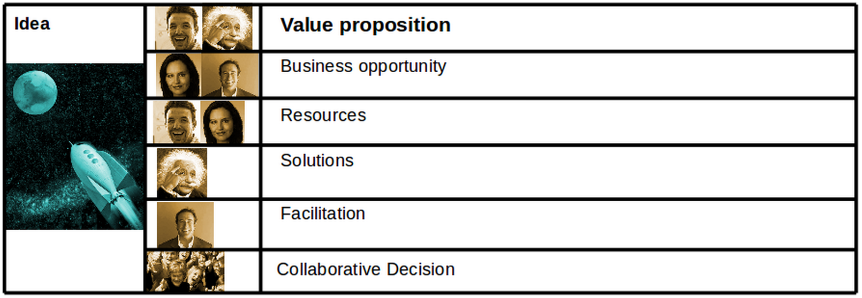
\includegraphics[width=1\textwidth]{pitch_card_original}
    \caption{Callaghan Innovation's design for a Pitch Card describes an idea with the following Pitch Points: Value Proposition (Any role, describing the idea's value), Business Opportunity (Challenger), Resources (Enabler), Solutions (Solver), Facilitation (Facilitator), Collaborative Decision (Any role, voting on the idea).}
    \label{fig:pitch_card_original}
\end{figure}

\subsection{Collaboration Conceptualisation}
Collaboration on PitchHub is actioned through users making suggestions and comments on these Pitch Points. This is ultimately how PitchHub offers the explicit support of collaboration between roles. Collaboration on PitchHub can be seen as a negotiation, where Pitch Card initiator's describe the idea, and suggestions from the community on the various Pitch Points are then accepted of rejected by the initiator. Accepted suggestions then update the Pitch Point, while rejected Pitch Points just serve as a record of the discussion. Beyond this negotiation of content, collaboration on PitchHub also features negotiation of visibility of content. Figure \ref{fig:pitch_card_original_collaboration} displays an example of a PitchCard view from the initiator's view.
\begin{figure}[ht]
    \centering
    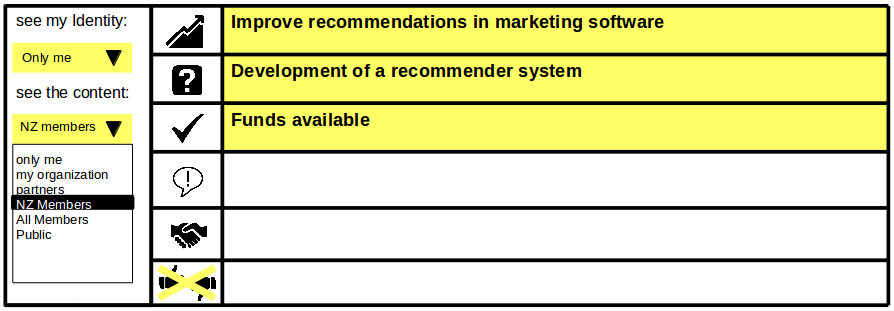
\includegraphics[width=1\textwidth]{pitch_card_original_collaboration}
    \caption{Callaghan Innovation's design for a Pitch Card's visibility scope as seen from a Pitch Card initiator's view.}
    \label{fig:pitch_card_original_collaboration}
\end{figure}

\section{Methodology}
The software methodology adopted in this project has been an agile, iterative approach. Each iteration is approximately one week in length and consists of the following actions: requirements analysis, requirements validation, design, development, testing, and documentation. During the early stages of the project identifying all of the requirements was infeasible as this would have required large contiguous amounts of time, of which Callaghan Innovation would not have been able to provide. So in keeping with the agile approach requirements were gathered progressively during client meetings and through the already completed conceptual work.

\section{Functional Requirements}
\begin{itemize}
\item The prototype must fulfill the user flows specified by Callaghan Innovation (i.e. the actions that enable the innovation community to connect and co-create).
\item The prototype must be store data securely to establish trust with users, by knowing that their commercially sensitive data is safe.
\item The prototype must provide privacy controls over user content so that users can control the scope of disclosure.
\end{itemize}

\section{Non-functional Requirements}
\begin{itemize}
\item The prototype must be performant, enabling users to fluently use the platform without distraction.
\item The prototype must support a distributed architecture to enable PitchHub the ability to scale and store data in a geographically redundant configuration.
\end{itemize}